\documentclass[10pt,a4paper]{book}

\usepackage{mystyle}

\begin{document}
\begin{titlepage}
\begin{center}
\hrule
{ \huge \bfseries PHYSIC\AE\\  MATHEMATICA}\\[0.5cm]
\hrule
The Philosophy of Mathematics and Physics

\emph{Collaborators:}\\
\begin{tabular}[center]{ccr@{@}l}
    Michael Schmidt & University of Colorado at Boulder & Michael.Schmidt & Colorado.EDU\\
    %Bryan Kaufman & University of Colorado at Boulder & Bryan.Kaufman & Colorado.EDU \\
\end{tabular}

\begin{figure*}[!h]
    \centering
	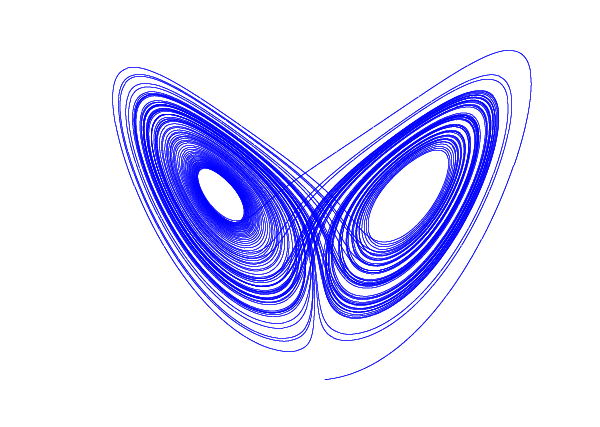
\includegraphics[scale=0.60]{./attractor.png}
\end{figure*}

\vfill
{\large \today}\\

This project is freely available at:\\
\url{http://github.com/schmidmt/Physicae-Mathematica}

\end{center}

\vfill


\end{titlepage}


%$Id: coverdetails.tex 6 2009-04-23 02:25:09Z schmidmt $%

\begin{center}
\begin{verbatim}
	Copyright (C)  2009 Michael Schmidt.
	Permission is granted to copy, distribute and/or modify this document
	under the terms of the GNU Free Documentation License, Version 1.3
	or any later version published by the Free Software Foundation;
	with no Invariant Sections, no Front-Cover Texts, and no Back-Cover Texts.
	A copy of the license is included in the section entitled "GNU
	Free Documentation License".
\end{verbatim}
\end{center}


\begin{center}
	\emph{Thanks To:}
\end{center}


\phantomsection
\tableofcontents

\frontmatter
\subsection*{Introduction}
\addcontentsline{toc}{subsection}{Introduction}
	\indent
	I began writing this book while attending the University of Colorado at Boulder.
	I'm writing this to help solidify my understanding of physics.
	My idea is if I am able to explain the concepts and mathematics behind physical theories then I understand them myself.
	This is not meant to be an introduction but simply a review of what is covered in an undergraduate curriculum.
	Hope you enjoy.\\
	\begin{flushright}
    \includegraphics[scale=0.1]{Signature.jpg}
	\end{flushright}


\startsoln

\mainmatter
\part{Mathematics}
\chapter{Introduction}
    \begin{quote}
        Mathematicians are people who would rather think than work.\newline
        \flushright{--David Grant}
    \end{quote}

    \bigskip

    First we shall start off with a definition:
    \begin{defn}
       \index{Abstraction}
       \underline{\emph{Abstraction}} is the process of producing a concept not associated with a specific instance.
    \end{defn}
    Why do we want this?
    Well it's simple, we would like to figure out how to build up concepts to permit us to predict, discover, and create new ideas.
    By grouping specific instances into concepts we can apply what we learn to a plethora of instances not just one.
    Also, we can use what other people have thought of and apply it to another instance without redoing the thinking.
    Besides, by abstracting we may discover new ideas which we could have never discovered otherwise.
    
    This brings us to our first main topic, mathematics.
    Mathematics is a philosophy used to bring together a vast number of topics into one topic so similarities between ideas may be exploited to discover the most elegant solution.
    For instance, ideas from calculus can be applied to geometry to analyze how shapes are, for lack of a better word, shaped.
    In regards to the quote above, math is a tool used to prevent "brute forcing" a solution.
    By "brute forcing" I mean trying every since possibility, basically guess and check with no direction at all.
    That would talk too much time.
    Remember if we can figure out a way to think of an problem in the most abstract we can more easily figure out the best way to solve it.

    So we start our endeavor first by ascertaining an idea of how to connect ideas.
    This topic is what we have come to call logic.

    \lipsum

\chapter{Logic}

\begin{bibunit}
  \nocite{Richmond2004Discrete}
  \nocite{Goldfarb2003Deductive}

  \section{Introduction}

Logic stems from the ancient Greek word \greek{lo'goc} (l\'{o}gos), which means \emph{that which is though or said}.
The reason we bring this up now is logic underpins all of mathematics.
More formally, we say mathematics is a formal system.
We will discuss what a formal system is later (see ~\ref{defn:formalSystem}) but for now, think of it as a construction of rules all logically compatible and built on a logical foundation.

Using a logical foundation allows us to trust the tools we will build.
Without this, we could not be sure when our math worked and tells us something true or something false.




\input{mathematics/logic/intro/statement}
\input{mathematics/logic/intro/negation}
\input{mathematics/logic/intro/conjunction}
\input{mathematics/logic/intro/disjunction}
\input{mathematics/logic/intro/conditional}
\input{mathematics/logic/intro/grouping}



  \putbib
\end{bibunit}

\chapter{Set Theory}

\def\firstcircle{(0,0) circle (3cm)}
\def\secondcircle{(0:4cm) circle (3cm)}

\colorlet{circle edge}{blue!50}
\colorlet{circle area}{blue!20}

\tikzset{filled/.style={fill=circle area, draw=circle edge, thick},
    outline/.style={draw=circle edge, thick}}

\begin{center}
% Set A and B
\begin{tikzpicture}
    \begin{scope}
        \clip \firstcircle;
        \fill[filled] \secondcircle;
    \end{scope}
    \draw[outline] \firstcircle node {$A$};
    \draw[outline] \secondcircle node {$B$};
    %\node[anchor=south] at (current bounding box.north) {$A \cap B$};
\end{tikzpicture}
\end{center}

\section{Introduction}
Here we are at the beginning of the mathematics specific content.
Before we get to deep into more complex topics, let us start with what may be considered the most primitive area of mathematics: set theory.
Like most theories, we wouldn't bother having a whole theory for something not punctuated by subtleties.
So we begin as we do with defining what we're talking about; but what is a set?

Naively, we usually say a set is a collection\footnote{I say collection since group is already taken.} of things.
Why is this naive?
You'll see in section~\ref{set:russellsparadox}.

\section{A First Pass At Set Theory}
For out first pass of set theory we will begin with \textbf{Na\"ive Set Theory}, or \textbf{NST}, ignoring future issues for the sake of building a foundational understanding.

\begin{defn}{Naive Set Theory}
  A \textbf{set} is a collection of items.
  It does not matter, for now, what the items are.
\index{element}
  If a particular item, say $a$, is in a set, say $A$, we call $a$ an \textbf{element} of $A$ or we say $a$ is in $A$.
  The boolean operator for establishing membership is $\in$, where $a \in A$ if and only if $a$ is an element of $A$.

  A set is usually denoted as a capitol Roman character.
  Later, we will decorate other symbols which are sets but have additional properties which make them easier to identify.
  To notate the set $A$ with elements $a,b,c$, we write:
  $$
    A = \left\{ a, b, c\right\}.
  $$
\end{defn}

Since any collection can be subdivided into other collections it is useful to make the notion of a \textbf{subset} strict.
To exemplify this, imagine two sets $A$ and $B$.
If each element of $A$ is in $B$ then $A$ is contained within $B$ or, in other words, $A$ is a subset of $B$.
To make this formal, the definition of a subset is as follows:
\begin{defn}{Subset}
  Suppose $A$ and $B$ are two sets.
  For each $a$ if $a$ is in $A$ and it is also in $B$ then $A$ is a \textbf{subset} of $B$.
  Symbolically this case is represented as $A \subset B$.
  Formally, this is represented by:
  $$
    \forall a \left\{ a \in A \implies a \in B \right\}  \Leftrightarrow A \subset B.
  $$
\end{defn}

Having a concept of a subset, we can now define the power set of a set.
\begin{defn}{Power Set}
  Let $A$ be a set.
  The \textbf{power set} of $A$, or $\mathcal{P}(A)$, is the set of all subsets of $A$.
  Formally, this is defined by:
  $$
    \forall x \left\{ x \in \mathcal{P}(A) \iff x \subset A \right\}.
  $$
\end{defn}

If two sets are mutually subsets of each other we say the sets are equivalent.
\begin{defn}{Set Equality}
  Suppose $A$ and $B$ are two sets.
  If $A \subset B$ and $B \subset A$ then $A$ and $B$ are \textbf{equal}, or $A = B$.
\end{defn}
This might at first seems a bit strange as the set $\left\{ a, a, b\right\}$ is the same as the set $\left\{ a, b \right\}$.
In this way, a set with repeated elements or elements in different orders are considered the same.
Later we will discuss different types of objects which do retain these qualities.

We may combine two sets in two distinct ways: we could group everything together, or we could select just the common elements.
The first way, grouping everything together is called the union of two sets as more precisely defined here:
\begin{defn}{Union}
\nomenclature{Union}{The union of two sets is the set of elements in both sets}
  Suppose $A$ and $B$ are two sets.
  The \textbf{union} of $A$ and $B$ is the set of all elements in at least one of the two sets.
  This is symbolically represented as $A \union B$ and is defined by the following sentence:
  $$
  \forall a \left\{ a \in A \union B \iff (a \in A \lor a \in B) \right\}.
  $$
  Using set builder notation, it can be defined as follows:
  $$
    A \union B =  \left\{ a | a \in A \lor a \in B \right\}.
  $$
\end{defn}

For the second way to combine two sets we only collect those elements which are in both sets.
We call this the \textbf{intersection} of two sets.
Formally, this is defined by:
\begin{defn}{Intersection}
\nomenclature{Intersection}{The intersection of two sets is the set of common elements}
  Suppose $A$ and $B$ are two sets.
  The \textbf{intersection} of $A$ and $B$ is the set of all elements at both sets.
  This is symbolically represented as $A \intersection B$ and is defined by the following sentence:
  $$
  \forall a \left\{ a \in A \intersection B \iff (a \in A \land a \in B) \right\}.
  $$
  Using set builder notation, it can be defined as follows:
  $$
    A \intersection B =  \left\{ a | a \in A \land a \in B \right\}.
  $$
\end{defn}


\subsection{Russell's Paradox}
Russell's Paradox is a simple proof that NST is inconsistent.
The proof is a follows: Imagine you have a set which 

$$
  \exists y \forall x (x \in y \iff P(x))
$$
and if $P(x) = x \notin x$, then
$$
  y \in y \iff y \notin y
$$
which means \textbf{NST} is inconsistent.

\section{Zermelo-Fraenkel Set Theory}

Zermelo-Frakenkel Set Theory, like any formal theory, is based in a set of axioms.

\subsection{The Axioms}
\begin{axiomset}
    \begin{center}
        \textbf{Zermelo--Fraenkel set theory with the axiom of choice}
    \end{center}
    \begin{axiom}
        Axiom of Extensionally:
        \begin{equation}
          \forall x \forall y [ \forall z ( z \in x \Leftrightarrow z \in y) \Rightarrow x = y ]
        \end{equation}
    \end{axiom}
    \begin{axiom}
        Axiom of Regularity:
        \begin{equation}
          \forall x [ \exists a ( a \in x ) \Rightarrow \exists y ( y \in x \land \neg \exists z ( z \in y \land z \in x ))]
        \end{equation}
    \end{axiom}
\end{axiomset}



\section{Formulation}
    Von Neumann universe


\chapter{Topology}


\chapter{The Numbers}


\chapter{Algebra}


\chapter{Linear Algebra}

\chapter{Analysis}

\lipsum

\chapter{Complex Analysis}

\chapter{Ordinary Differential Equations}

\section{1st Order}

\section{2nd Order}

\section{Systems of 1st Order Differential Equations}



\chapter{Partial Differential Equations}

\chapter{Differential Geometry}

\chapter{Fourier Analysis}

\chapter{Combinatorics}

\chapter{Probability}

\chapter{Statistics}

\chapter{Numerical Analysis}

\lipsum



\part{Physics}
\chapter{General Statements}
    \begin{bibunit}
	\section{Noether's Theorem: Conservation Laws}

\label{sec:noether}
\begin{thm}
	For every symmetry there corresponds a conserved quantity.\cite{Noether2005Invariant}\index{Noether's Theorem}
\end{thm}
\lipsum

	\section{Lagrangian and Hamiltonian Dynamics}


	\putbib
	\end{bibunit}

\chapter{Classical Mechanics}
	\section{Introduction}
	Classical Dynamics Introduction...
	
	\section{Lagrangian and Hamiltonian Dynamics}

\lipsum

	\section{Newtonian Dynamics}
	\begin{equation}
		\vect{F} = \frac{d}{d t} (m \vect{v}) = \dot{\vect{P}}
		\label{Newton's Force equation}
	\end{equation}


	

\chapter{Electrodynamics}

\lipsum

	

\chapter{Quantum Dynamics}

\lipsum

\chapter{Plasma Physics}

\lipsum

\chapter{Particle Physics}

\lipsum

\chapter{Computational Physics}

\lipsum



\part{Computer Science}



\stopsoln

\part{Reference}

\appendix
\chapter{Solutions}
%\addcontentsline{toc}{Section}{Solutions}
\putsoln

\backmatter
\chapter{Editor Guidelines}
\begin{description}
    \item{Layout} \hfill \\
    \begin{enumerate}
        \item Each chapter or sections must be contained in a separate file and included in the main physicae.tex file.
    \end{enumerate}
    \item{Theorems, Lemma, Examples} \hfill \\
    \begin{enumerate}
        \item Each theorem or lemma must have a proof associated with it.
        \item Each example must have a solution associated with it.
    \end{enumerate}
\end{description}

\chapter{GNU Free Document License}
\verbatiminput{appendixes/fdl-1.3.txt}


\addcontentsline{toc}{Section}{List of Figures and Tables}
\listoffigures
\listoftables

\addcontentsline{toc}{Section}{Symbols and Nomenclature}
\printnomenclature


\addcontentsline{toc}{Section}{Index}
\printindex


\end{document}
